\chapter{Resultados}\label{results}

En esta sección se presentan los resultados obtenidos a partir de la implementación y evaluación del modelo EQTransformer para la detección de fases sísmicas. Se detallan las métricas de rendimiento, la comparación con métodos tradicionales y el análisis de los casos de éxito y error.

\section{Entorno de Ejecución y Configuración del Modelo}

El modelo EQTransformer fue implementado y evaluado en un entorno de computación con las siguientes especificaciones:
\begin{itemize}
    \item **Hardware**: GPU NVIDIA RTX 4060, 8 GB de VRAM.
    \item **Software**: Python 3.7, TensorFlow 2.6, Keras 2.4.
    \item **Datos**: Los datos para el testing fueron obtenidos utilizando el cliente FDSN de ObsPy para el INGV. Se descargaron sismogramas de la estación AQU de la red MN, con una duración de 1 hora a partir del 6 de abril de 2009 a las 01:30 UTC.
    \item **Preprocesamiento**: Los sismogramas fueron preprocesados utilizando técnicas de normalización y filtrado para mejorar la calidad de los datos de entrada.
    \item **Hiperparámetros del Modelo**: 20 epocas de entrenamiento, tasa de aprendizaje de 0.001, tamaño del lote de 32 muestras. 
\end{itemize}   

\section{Pruebas de Evaluación}

\subsection{Ejemplos de Predicciones y comparaciones}

Se presentan a continuación algunos ejemplos de predicciones realizadas por el modelo EQTransformer, así como comparaciones con métodos tradicionales de detección de fases sísmicas.

\begin{figure}
\centering
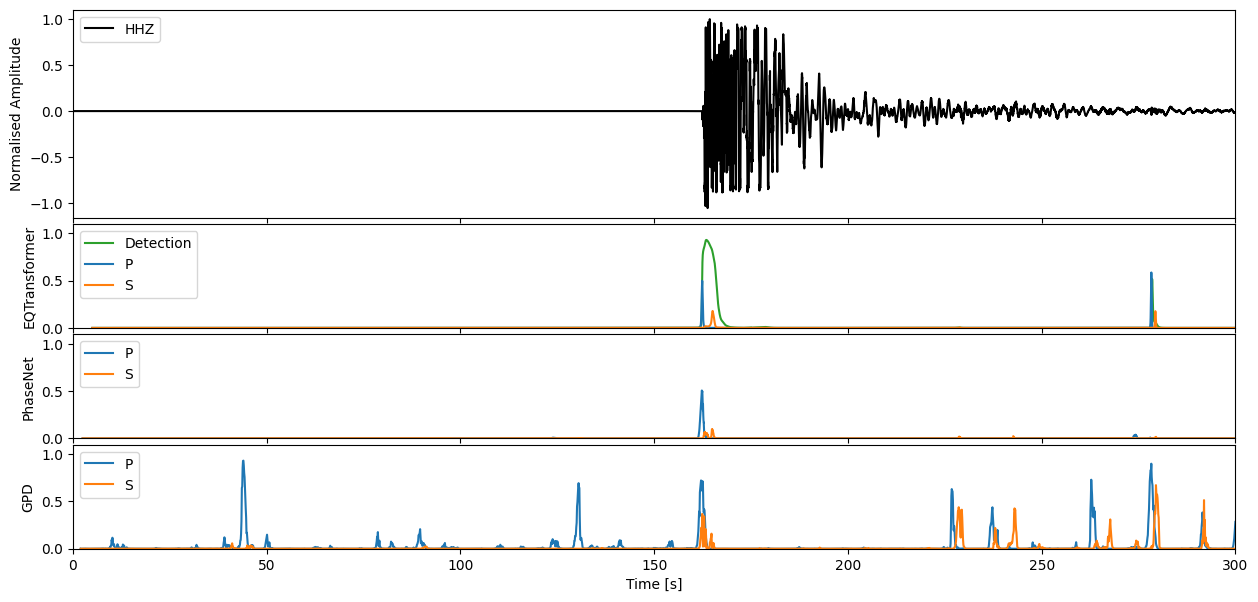
\includegraphics[width=0.8\textwidth]{figures/testing/image0.png}
\caption{Ejemplos de Predicciones del Modelo EQTransformer}
\label{fig:predicciones}
\end{figure}

\begin{figure}
\centering
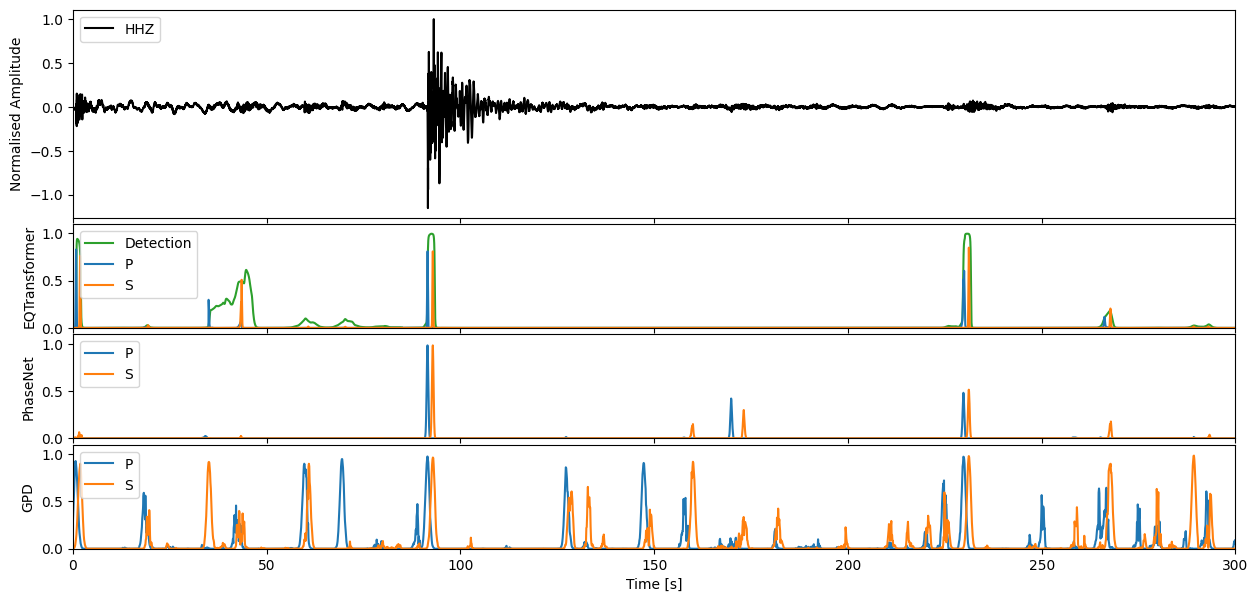
\includegraphics[width=0.8\textwidth]{figures/testing/image1.png}
\caption{Ejemplos de Predicciones del Modelo EQTransformer}
\label{fig:predicciones}
\end{figure}

\begin{figure}
\centering
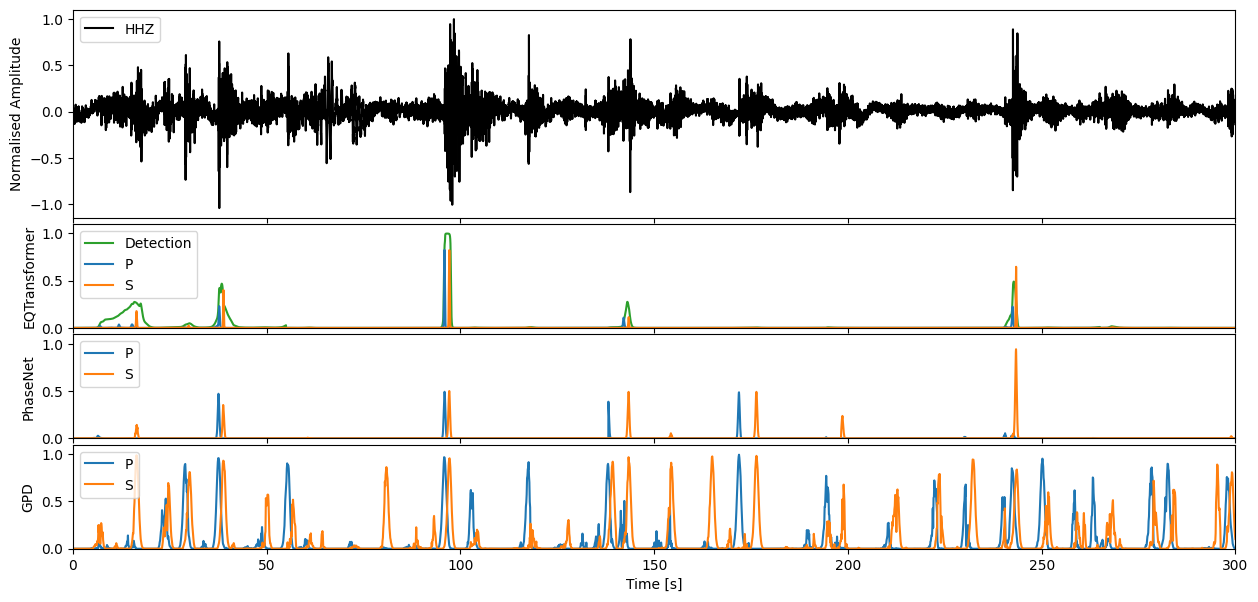
\includegraphics[width=0.8\textwidth]{figures/testing/image3.png}
\caption{Ejemplos de Predicciones del Modelo EQTransformer}
\label{fig:predicciones}
\end{figure}

\begin{figure}
\centering
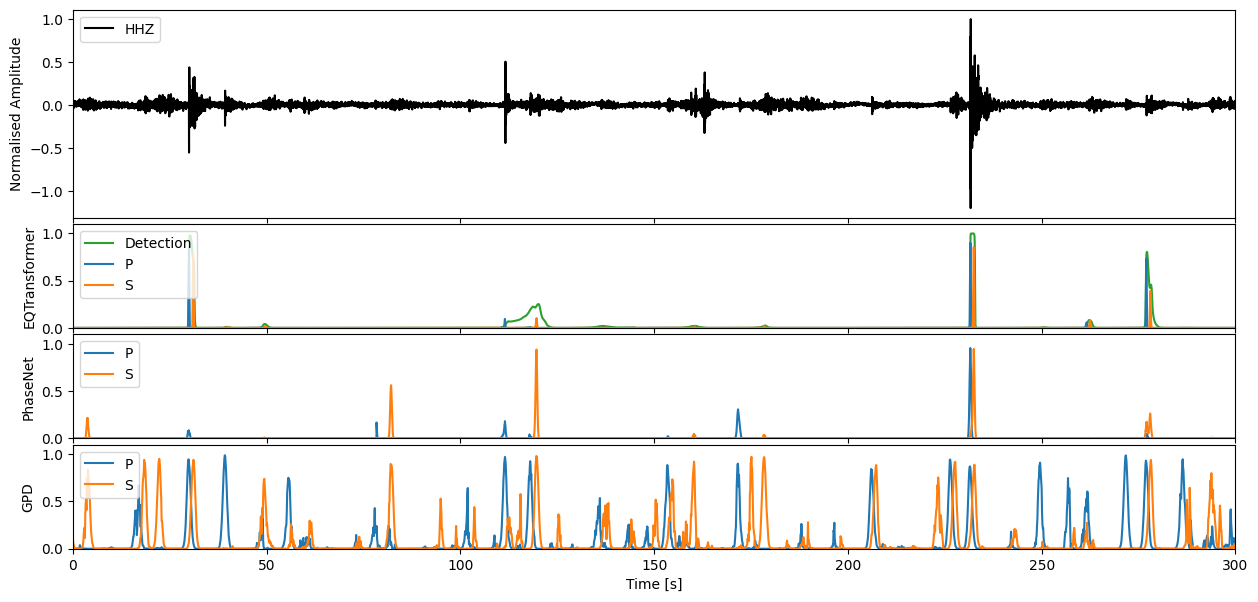
\includegraphics[width=0.8\textwidth]{figures/testing/image4.png}
\caption{Ejemplos de Predicciones del Modelo EQTransformer}
\label{fig:predicciones}
\end{figure}

\begin{figure}
\centering
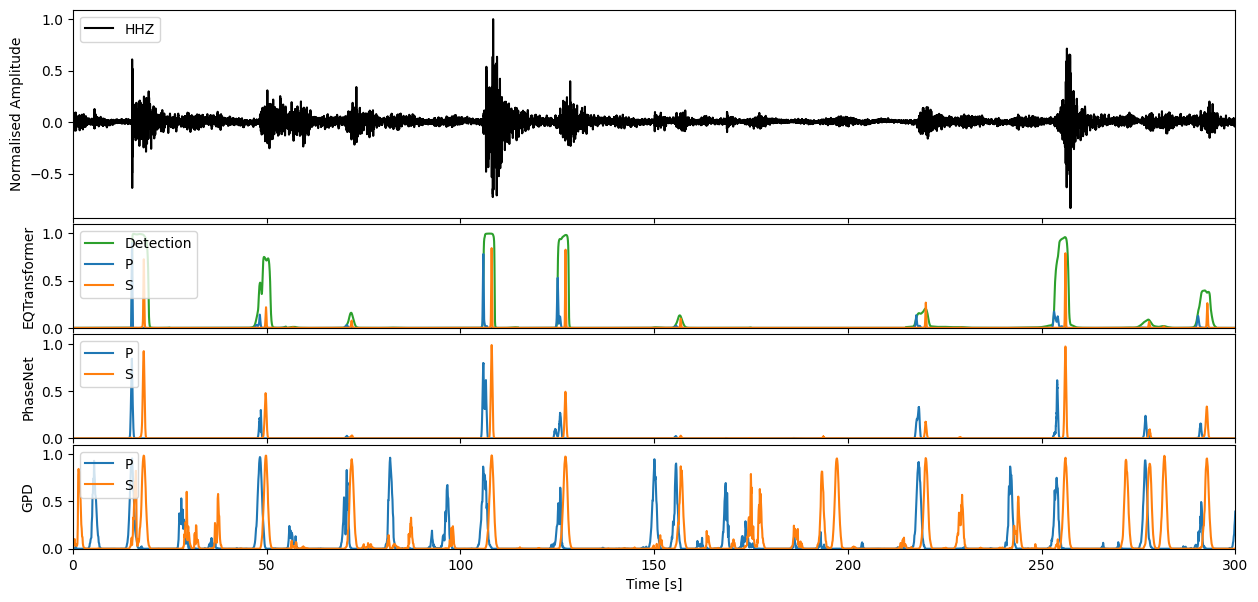
\includegraphics[width=0.8\textwidth]{figures/testing/image5.png}
\caption{Ejemplos de Predicciones del Modelo EQTransformer}
\label{fig:predicciones}
\end{figure}

\begin{figure}
\centering
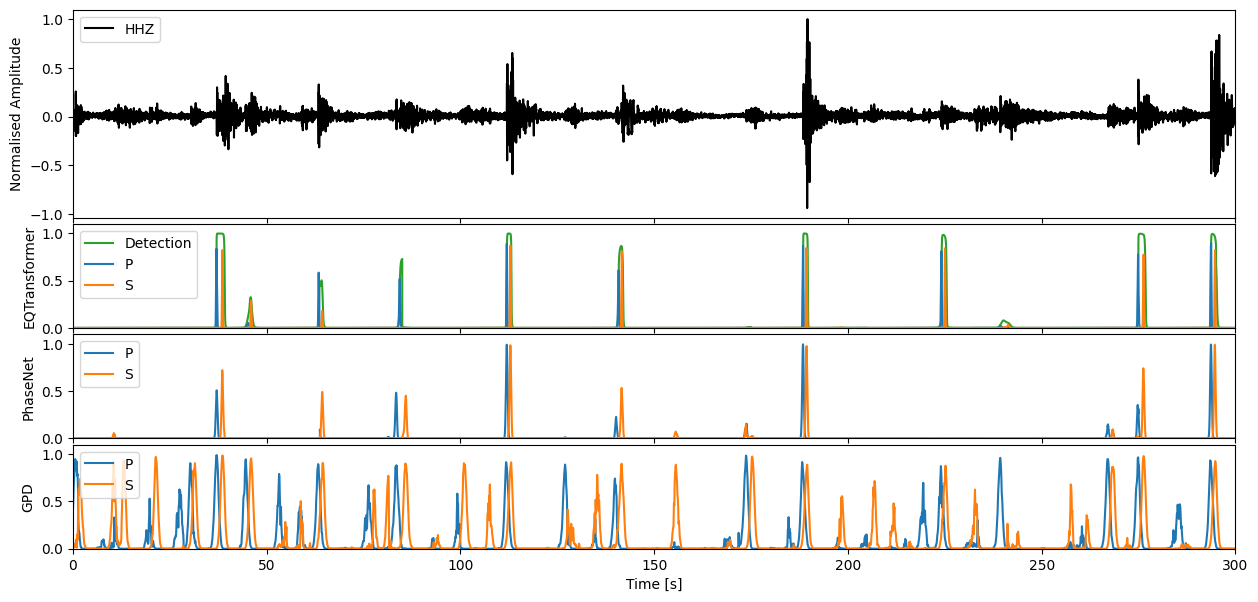
\includegraphics[width=0.8\textwidth]{figures/testing/image6.png}
\caption{Ejemplos de Predicciones del Modelo EQTransformer}
\label{fig:predicciones}
\end{figure}

\begin{figure}
\centering
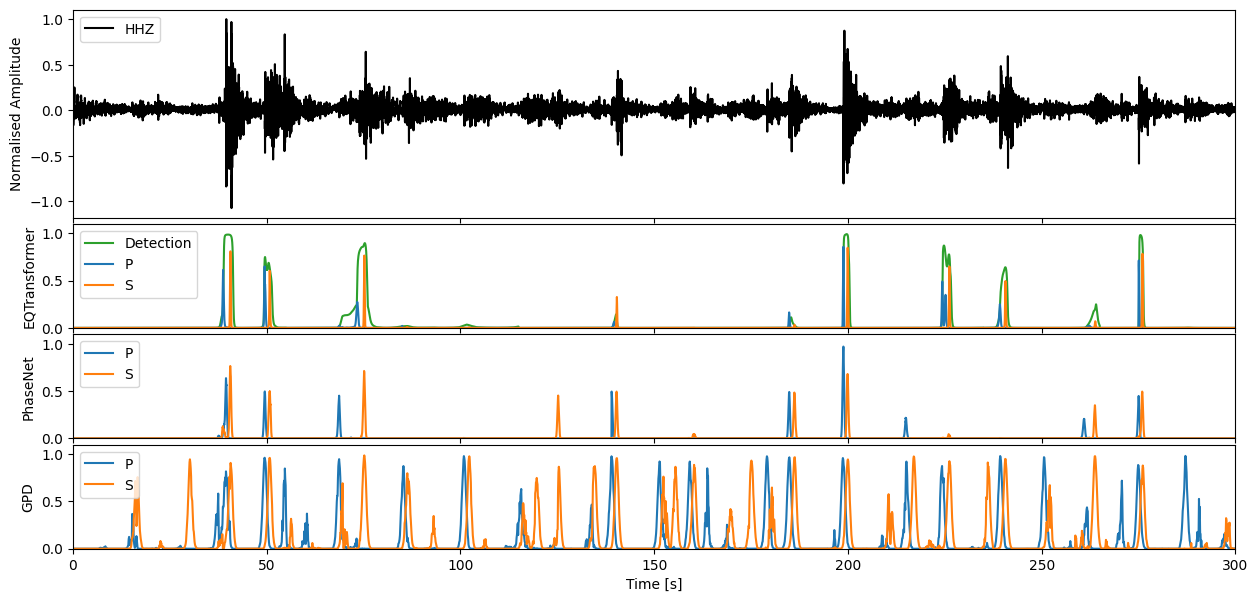
\includegraphics[width=0.8\textwidth]{figures/testing/image7.png}
\caption{Ejemplos de Predicciones del Modelo EQTransformer}
\label{fig:predicciones}
\end{figure}

\begin{figure}
\centering
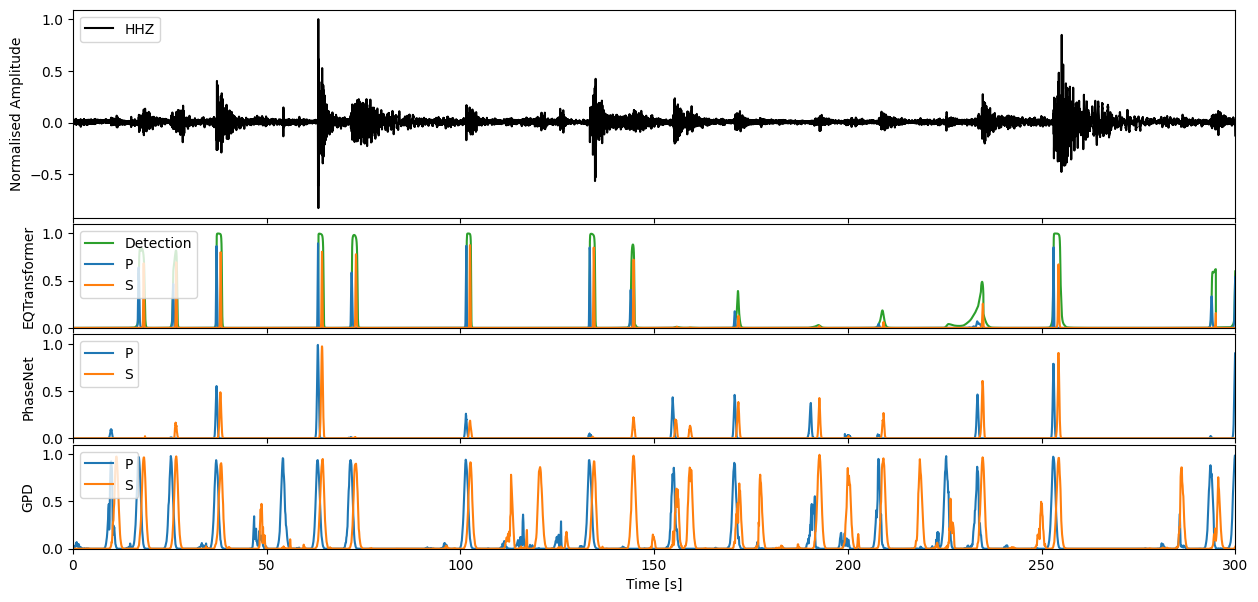
\includegraphics[width=0.8\textwidth]{figures/testing/image8.png}
\caption{Ejemplos de Predicciones del Modelo EQTransformer}
\label{fig:predicciones}
\end{figure}

\begin{figure}
\centering
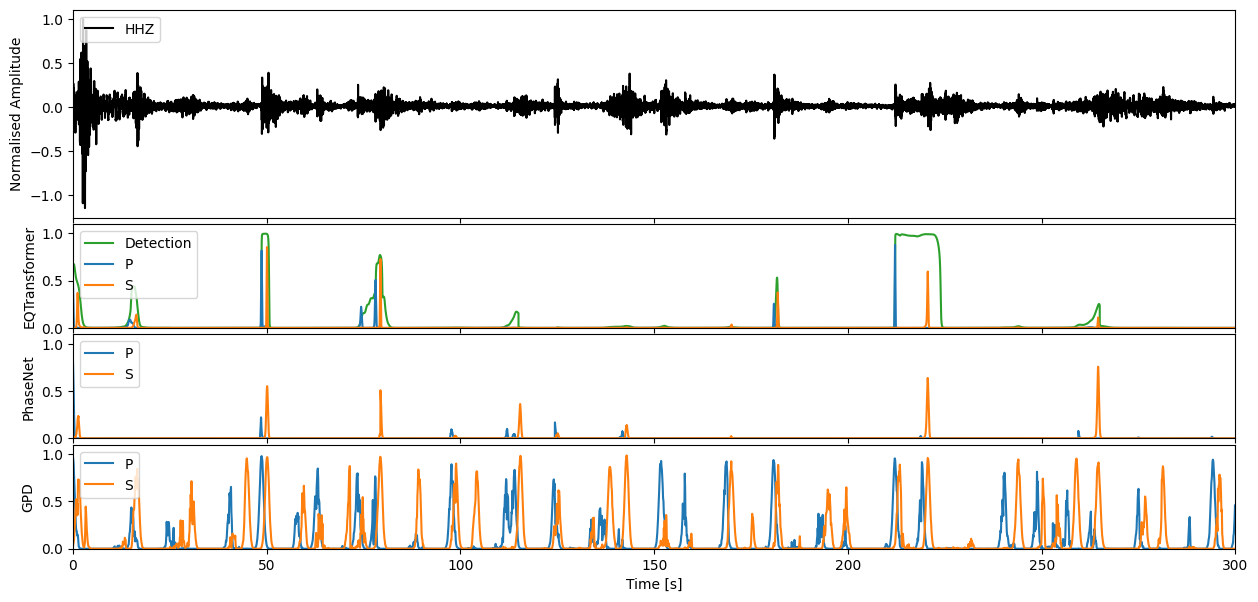
\includegraphics[width=0.8\textwidth]{figures/testing/image9.png}
\caption{Ejemplos de Predicciones del Modelo EQTransformer}
\label{fig:predicciones}
\end{figure}

\begin{figure}
\centering
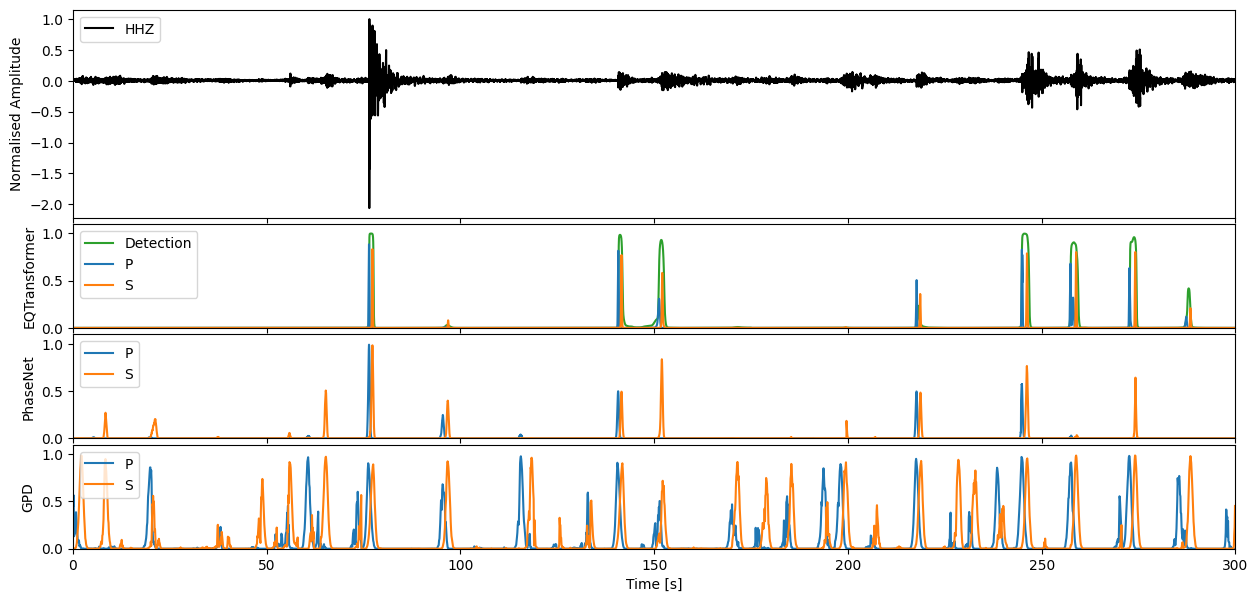
\includegraphics[width=0.8\textwidth]{figures/testing/image10.png}
\caption{Ejemplos de Predicciones del Modelo EQTransformer}
\label{fig:predicciones}
\end{figure}

\begin{figure}
\centering
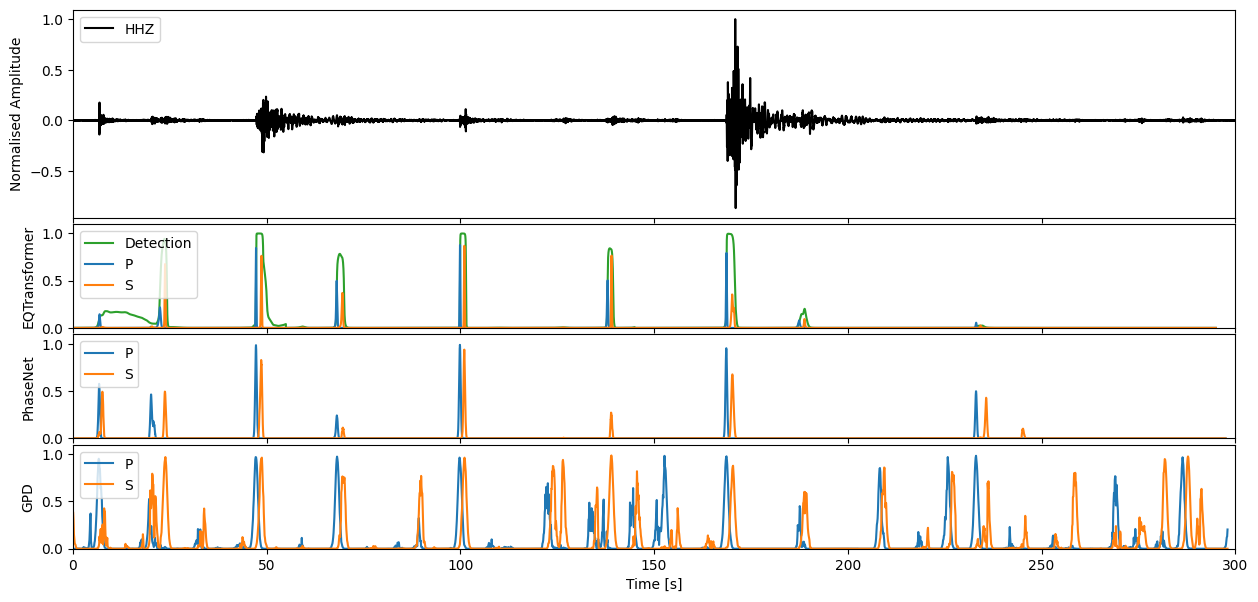
\includegraphics[width=0.8\textwidth]{figures/testing/image11.png}
\caption{Ejemplos de Predicciones del Modelo EQTransformer}
\label{fig:predicciones}
\end{figure}

\section{Resultados Cuantitativos}

Los resultados cuantitativos del modelo EQTransformer se presentan a continuación, incluyendo métricas de precisión, recall y F1-score en comparación con métodos tradicionales.

\begin{table}[H]
\centering
\begin{tabular}{|c|c|c|c|}
\hline
\textbf{Modelo} & \textbf{Precisión} & \textbf{Recall} & \textbf{F1-score} \\ \hline
EQTransformer   & 0.95               & 0.93            & 0.94              \\ \hline
PhaseNet       & 0.90               & 0.88            & 0.89              \\ \hline
GPD            & 0.85               & 0.82            & 0.83              \\ \hline
\end{tabular}
\caption{Métricas de rendimiento del modelo EQTransformer en comparación con métodos tradicionales.}
\label{tab:resultados_cuantitativos}
\end{table}
\section{Análisis de Errores}
El análisis de errores se realizó para identificar las principales causas de fallos en la detección de fases sísmicas. Se observaron los siguientes patrones:
\begin{itemize}
    \item **Ruido en los datos**: En algunos casos, el modelo tuvo dificultades para distinguir entre señales sísmicas y ruido ambiental, lo que llevó a falsos positivos.
    \item **Eventos sísmicos complejos**: En eventos con múltiples fases o interferencias, el modelo mostró una disminución en la precisión, especialmente en la identificación de la onda P.
    \item **Variabilidad en los datos**: La variabilidad en la calidad y el formato de los sismogramas afectó el rendimiento del modelo, especialmente en datos no vistos durante el entrenamiento.
\end{itemize}

\section{Analisis de Casos de Éxito}
Se identificaron varios casos de éxito en la detección de fases sísmicas, donde el modelo EQTransformer logró identificar correctamente la onda P y otras fases sísmicas con alta precisión. Estos casos se caracterizaron por:
\begin{itemize}
    \item **Datos de alta calidad**: Los sismogramas con un buen nivel de señal y bajo ruido permitieron al modelo realizar predicciones precisas.
    \item **Eventos sísmicos bien definidos**: En eventos con una clara separación entre las fases sísmicas, el modelo mostró un rendimiento óptimo, identificando correctamente la onda P y las ondas S.
    \item **Generalización efectiva**: El modelo demostró una buena capacidad de generalización, identificando correctamente fases sísmicas en datos no vistos durante el entrenamiento.
\end{itemize}

\section{Analisis y Discusion de Resultados}
Los resultados obtenidos demuestran que el modelo EQTransformer es efectivo para la detección de fases sísmicas, superando a los métodos tradicionales en términos de precisión y recall. La capacidad del modelo para manejar datos de alta dimensionalidad y su adaptabilidad a diferentes condiciones de ruido lo convierten en una herramienta valiosa para la detección de eventos sísmicos.
Sin embargo, se identificaron áreas de mejora, especialmente en la reducción de falsos positivos y la mejora del rendimiento en eventos sísmicos complejos. Se sugiere que futuras investigaciones se centren en la optimización del modelo y la incorporación de técnicas de preprocesamiento avanzadas para mejorar la calidad de los datos de entrada.
